\documentclass[mathserif]{beamer}
%\documentclass{beamer}
\usetheme{Luebeck}
\usecolortheme{spruce}
\usecolortheme{rose}
\usepackage{amsmath,verbatim}
\usepackage{listings}
\usepackage[english]{babel}
%\usepackage{media9} % package for genuine embedding of movies
\usepackage{multimedia} % beamer package for calling external files and players
\setbeamercovered{transparent}

% media9 stuff for playing movies
%\newcommand{\includemovie}[3]{\includemedia[width=#1,height=#2,activate=pagevisible,deactivate=pageclose,addresource=#3,flashvars={src=#3 &autoPlay=true &loop=true &controlBarAutoHideTimeout=0 }]{}{VPlayer.swf}}

\newcommand{\trans}{\ensuremath{{}^\mathrm{T}}}
\newcommand{\eps}{\varepsilon}
\newcommand*{\approxdist}{\mathrel{\vcenter{\offinterlineskip
\vskip-.25ex\hbox{\hskip.55ex$\cdot$}\vskip-.25ex\hbox{$\sim$}
\vskip-.5ex\hbox{\hskip.55ex$\cdot$}}}}

\lstdefinelanguage{myR}
{
   language=R,
   otherkeywords={read.table, set.seed, head},
   deletekeywords={url,codes, t, dt, Call, formula,Q, R, on,by,hat,is,
col, set,start,end,deltat,zip},
   sensitive=true,
   breaklines=true,
   morecomment=[l]{\#},
   morestring=[b]",
   morestring=[b]',
   basicstyle =\ttfamily\small,
   keywordstyle=\bfseries,
   showtabs=false,
   showstringspaces=false,
   literate= {~}{$\sim$}{2},
   numberstyle=\sffamily\scriptsize,
   stepnumber=2
 }

\lstset{basicstyle=\ttfamily\color{blue}}

\begin{document}

\title{Spatially distributed stochastic kinetic models}
\author[Darren Wilkinson --- Statistics seminar, 5/2/16]{\textbf{\large Darren Wilkinson} \\
\url{@darrenjw}\\
\alert{\url{tinyurl.com/darrenjw}}\\
School of Mathematics \& Statistics\\Newcastle University, UK}
\date{Statistics Seminar\\Newcastle University\\5th February 2016}

\frame{\titlepage}

\section{Introduction}

\subsection{Outline}

\frame{
\frametitle{Talk outline}
\begin{itemize}
\item Chemical reaction networks
\item Discrete mass-action stochastic kinetics
\item Diffusion and the well-mixed assumption
\item Stochastic diffusion in 1D
\item Stochastic reaction-diffusion in 1D
\item Stochastic diffusion and reaction-diffusion in 2D
\item Filtering stochastic reaction-diffusion models?!
\end{itemize}
}

\subsection{Chemical reaction networks}


\frame{
\frametitle{Lotka--Volterra system}
Trivial (familiar) example from population dynamics (in reality, the
``reactions'' will be elementary biochemical reactions taking place
inside a cell)
%The running example through this talk will be a familiar example from population dynamics --- the Lotka--Volterra predator--prey system. We will regard it as a particular example of a broad class of nonlinear multivariate Markov jump processes known as \alert{stochastic kinetic models}
\begin{block}{Reactions}
\begin{align*}
X &\longrightarrow 2X \tag{prey reproduction}\\
X+Y &\longrightarrow 2Y \tag{prey-predator interaction}\\
Y &\longrightarrow \emptyset \tag{predator death}
\end{align*}
\end{block}
\begin{itemize}
\item $X$ -- Prey, $Y$ -- Predator
\item We can re-write this using matrix notation
% for the corresponding Petri net
\end{itemize}
}


\frame{
\frametitle{Forming the matrix representation}
\begin{block}{The L-V system in tabular form}
\begin{center}
\begin{tabular}{|c|c|rr|rr|rr|}\hline
& Rate Law &\multicolumn{2}{|c|}{LHS}&\multicolumn{2}{|c|}{RHS}&\multicolumn{2}{|c|}{Net-effect} \\
& $h(\cdot,c)$ & $X$&$Y$ & $X$&$Y$ & $X$&$Y$ \\ \hline
$R_1$ & $c_1 x$ & 1 & 0 & 2 & 0 & 1 & 0 \\
$R_2$ & $c_2 xy$ & 1 & 1 & 0 & 2 & -1 & 1 \\
$R_3$ & $c_3 y$ & 0 & 1 & 0 & 0 & 0 & -1 \\ \hline
\end{tabular}
\end{center}
\end{block}
%\pause
Call the $3\times 2$ net-effect (or \alert{reaction}) matrix $N$. The 
matrix $S=N'$ is the \alert{stoichiometry matrix} of the
system. 
Typically both are \alert{sparse}. 
%The SVD of $S$ (or $N$) is
%of interest for structural analysis of the 
%system dynamics...
}


\frame{
\frametitle{Stochastic chemical kinetics}
\begin{itemize}
\item $u$ species: $\mathcal{X}_1,\ldots,\mathcal{X}_u$, and $v$
reactions: $\mathcal{R}_1,\ldots,\mathcal{R}_v$
\item $\mathcal{R}_i:\ p_{i1}\mathcal{X}_1+\cdots+p_{iu}\mathcal{X}_u
\longrightarrow q_{i1}\mathcal{X}_1+\cdots+q_{iu}\mathcal{X}_u,\ 
i=1,\ldots,v$
\item In matrix form: $P\mathcal{X} \longrightarrow Q\mathcal{X}$ ($P$
and $Q$ are \alert{sparse})
\item $S=(Q-P)'$ is the \alert{stoichiometry matrix} of the system
\item $X_{jt}$: \# molecules of $\mathcal{X}_j$ at time
$t$. $X_t=(X_{1t},\ldots,X_{ut})'$
\item Reaction $\mathcal{R}_i$ has \alert{hazard} (or \alert{rate law}, or
\alert{propensity}) $h_i(X_t,c_i)$, where $c_i$ is a \alert{rate
parameter}, $c=(c_1,\ldots,c_v)'$,
$h(X_t,c)=(h_1(X_t,c_1),\ldots,h_v(X_t,c_v))'$ and the system evolves as a \alert{Markov jump process}
\item For \alert{mass-action stochastic kinetics},
\[
h_i(X_t,c_i) = c_i\prod_{j=1}^u\binom{X_{jt}}{p_{ij}},\quad i=1,\ldots,v
\]
\end{itemize}
}


\frame{
\frametitle{The Gillespie algorithm}
\small
\begin{enumerate}
\item Initialise the system at $t=0$ with rate constants
$c_1,c_2,\ldots,c_v$ and initial numbers of molecules for each
species, $x=(x_1,x_2,\ldots,x_u)'$.
\item For each $i=1,2,\ldots,v$, calculate $h_i(x,c_i)$ based on the
current state, $x$.
\item Calculate $h_0(x,c) \equiv \sum_{i=1}^v h_i(x,c_i)$, the
combined reaction hazard.
\item Simulate time to next event, $\tau$, as an $Exp(h_0(x,c))$ random
quantity, and put $t:=t+\tau$.
\item Simulate the reaction index, $j$, as a discrete random quantity
with probabilities $h_i(x,c_i)$ $/$ $h_0(x,c)$, $i=1,2,\ldots,v$.
\item Update $x$ according to reaction $j$. That is, put
$x:=x+S^{(j)}$, where $S^{(j)}$ denotes the $j$th column of the
stoichiometry matrix $S$.
\item Output $x$ and $t$.
\item If $t<T_{max}$, return to step 2.
\end{enumerate}
}



\frame{
\frametitle{The Lotka-Volterra model}
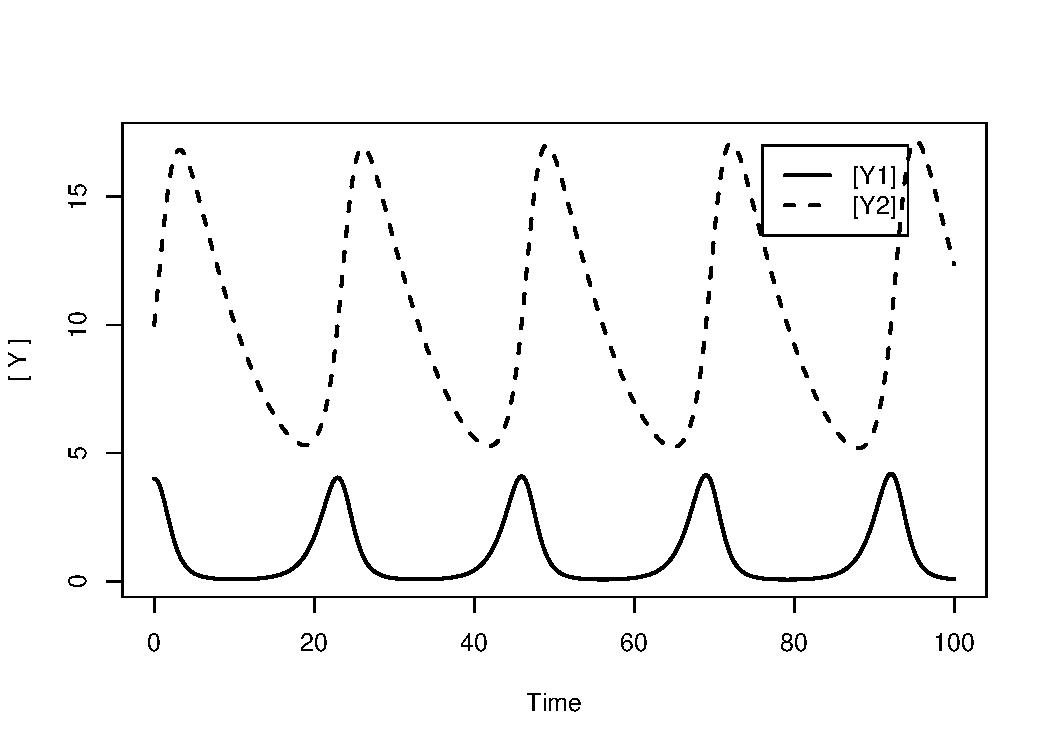
\includegraphics[width=5cm,clip=true]{ch06-lv-dynamics}
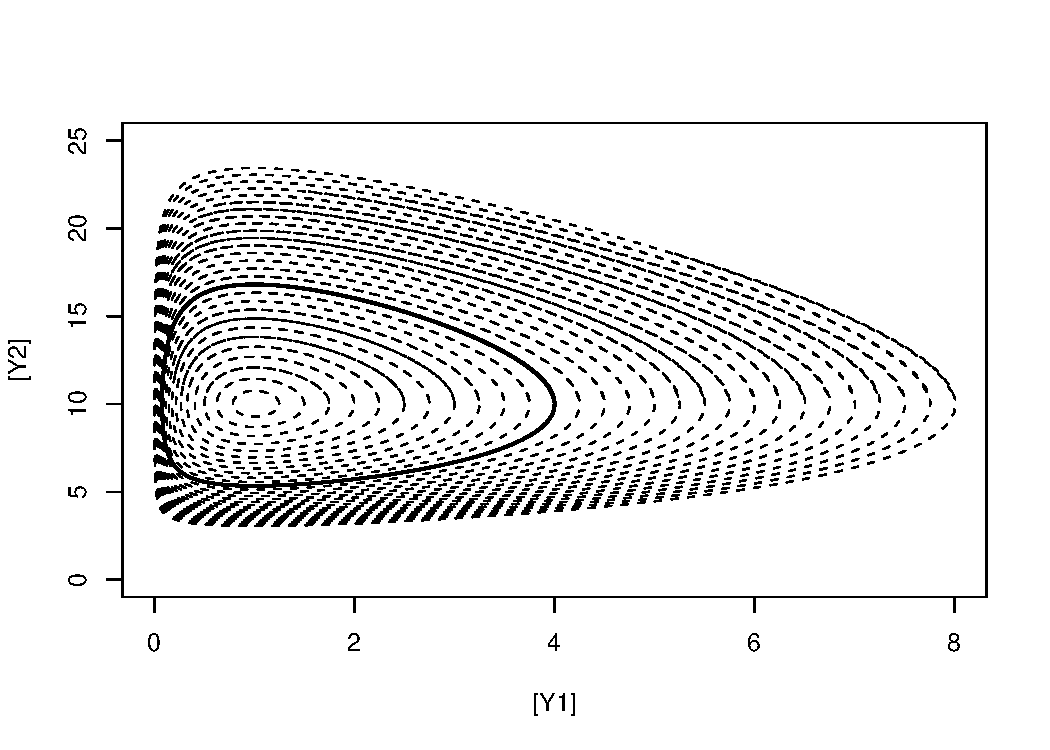
\includegraphics[width=5cm,clip=true]{ch06-lv-phase}
\\
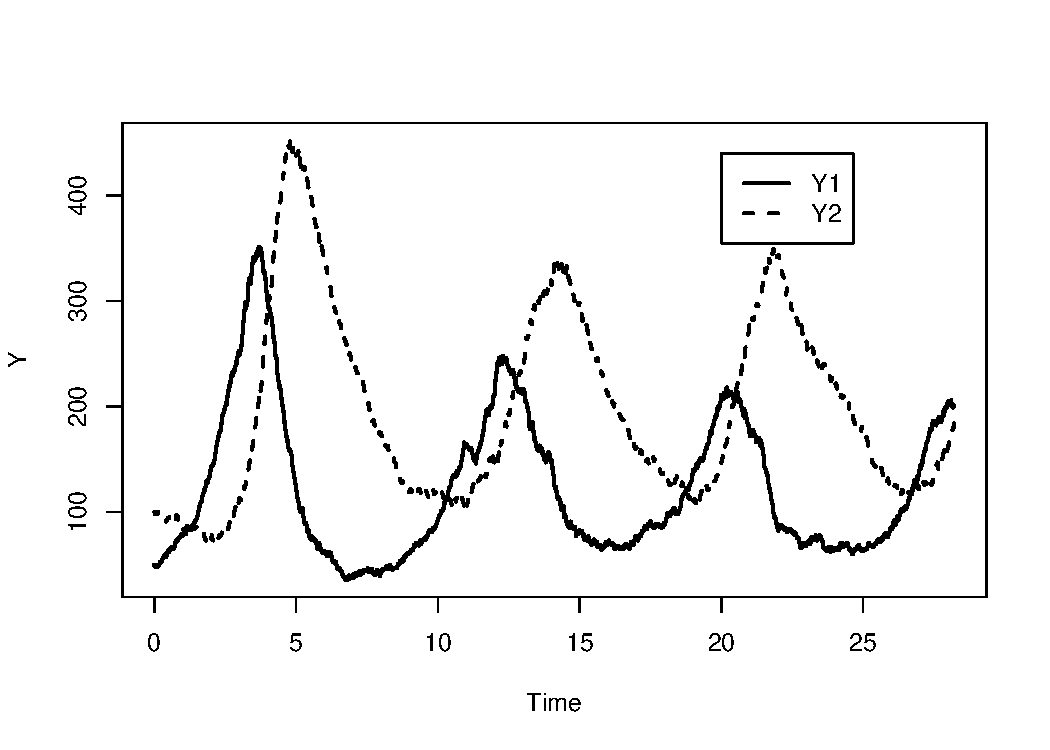
\includegraphics[width=5cm,clip=true]{ch06-stoch-lv}
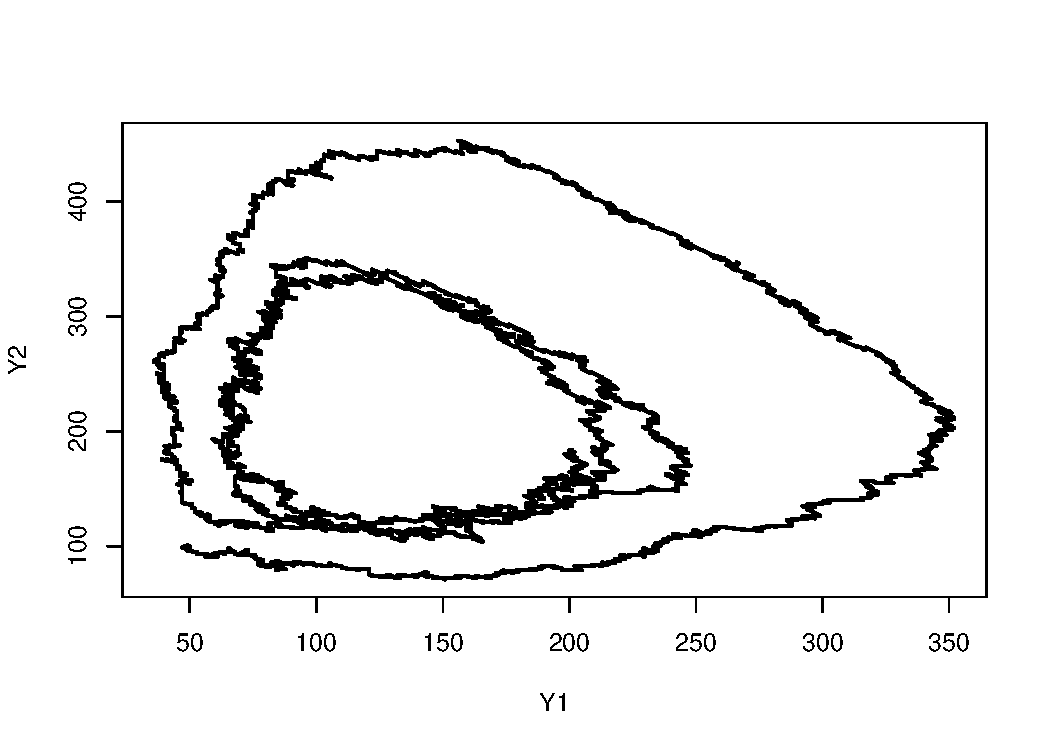
\includegraphics[width=5cm,clip=true]{ch06-stoch-lv-phase}
}

\subsection{The well-mixed assumption}


\frame{
\frametitle{The well-mixed assumption}
\begin{itemize}
\item The fundamental assumption underpinning the mass-action stochastic kinetic approach to modelling chemical reactions as a Markov jump process is that the hazard associated with any reaction event is \alert{constant}
\item It is this assumption of constant hazard which leads to exponential inter-arrival times of reaction events and all of the other algorithms commonly used for non-spatial modelling
\item However, it's pretty clear that molecules far apart will have a lower reaction hazard than molecules which are nearby
\item Mass-action kinetics assumes that molecular \alert{diffusion} is rapid relative to the time scales associated with the chemical \alert{reactions}
\item Evidence that this assumption is violated for some interesting intra-cellular processes
\end{itemize}
}


\section{Lattice models for diffusion and reaction diffusion}

\subsection{Stochastic molecular diffusion}

\frame{
\frametitle{Stochastic particle models}
\begin{itemize}
\item One approach to discrete stochastic modelling of reaction diffusion processes is to completely abandon the well-mixed framework and switch to modelling the position of every single molecule in space
\item Molecules can react when they ``collide'' (come within a threshold reaction distance)
\item Sophisticated statistical physics theory for describing the probabilistic behaviour of such processes, and complex algorithms for exact and approximate stochastic simulation of time course trajectories of the system evolution
\item Several free software implementations, with \alert{Smoldyn} being a notable example (Andrews et al, 2010)
\item Although useful for some problems, it's very difficult to implement, and exceptionally computationally intensive...
\end{itemize}
}


\frame{
\frametitle{Discrete stochastic models of diffusion}
\begin{itemize}
\item Let us begin by assuming that we can identify finite subvolumes of volume $V$ sufficiently small that the well-mixed assumption is valid
\item Note that we are regarding $V$ as fixed and \alert{not} (at this stage) thinking about taking any kind of continuum limit as, say, $V\longrightarrow 0$
\item Just consider a single species, $X$, which is well-mixed within each subvolume
\item However, molecules may be able to move (\alert{diffuse}) to an adjacent subvolume
\item It is clear that the \alert{rate} at which a particular molecule will diffuse to an adjecent subvolume must be \alert{constant}, due to the well mixed assumption
\end{itemize}
}

\subsection{Stochastic diffusion on a 1D lattice}

\frame{
\frametitle{Discrete stochastic diffusion on a 1D lattice}
\centerline{\includegraphics[height=0.3\textheight]{1d}}
\begin{itemize}
\item Assume a collection of $N$ subvolumes, labelled $1,2,\ldots,N$, each of volume $V$, arranged linearly so that a molecule in subvolume $i$ may diffuse to subvolume $i+1$ (and \emph{vice versa})
\item The \alert{diffusion rate} is $D$, so that the probability of a particular molecule in volume $i$ moving to volume $i+1$ in time $\delta t$ is $D\delta t$
\end{itemize}
}

\frame{
\frametitle{Stochastic kinetics of diffusion}
\centerline{\includegraphics[height=0.2\textheight]{1d}}
\begin{itemize}
\item We can think of diffusion events as ``reactions'':
\begin{align*}
{\cal X}_i &\longrightarrow {\cal X}_{i+1} \\
{\cal X}_i &\longrightarrow {\cal X}_{i-1} 
\end{align*}
\item There are 2 reactions per subvolume, so $2N$ reactions in total (for periodic boundary conditions)
\item This defines a Markov jump process which we can solve exactly or simulate using the Gillespie algorithm
\end{itemize}
}

\frame{
\frametitle{Simulating 1D diffusion}
\centerline{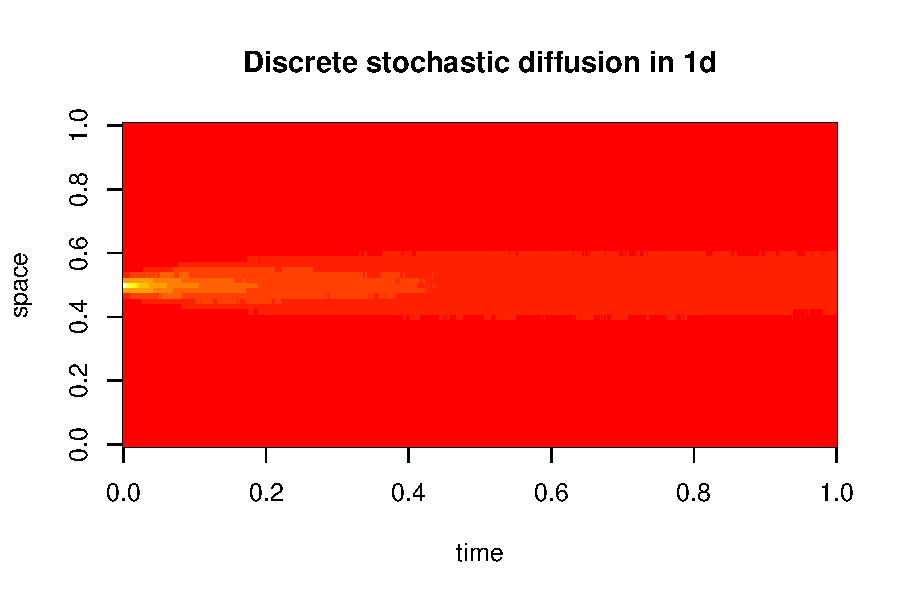
\includegraphics[height=0.8\textheight]{dsdiff1d}}
}

\frame{
\frametitle{SDE approximation of discrete stochastic diffusion}
\begin{itemize}
\item Let $X_{i,t}$ be the number of molecules (of $\cal X$) in volume $i$ at time $t$
\item Molecules leave volume $i$ at rate $2DX_{i,t}$ and enter at rate $D(X_{i-1,t}+X_{i+1,t})$
\item So for $\delta X_{i,t}=X_{i,t+\delta t}-X_{i,t}$ we have
\begin{align*} 
\operatorname{E}(\delta X_{i,t}) &\simeq D(X_{i-1,t}-2X_{i,t}+X_{i+1,t})\delta t\\
\operatorname{Var}(\delta X_{i,t}) &\simeq D(X_{i-1,t}+2X_{i,t}+X_{i+1,t})\delta t
\end{align*}
\item It is helpful to re-write the expectation using \alert{finite differences} notation
\end{itemize}
}

\frame{
\frametitle{Finite differences}
\begin{itemize}
\item Backshift operator, $B$, s.t. $BX_{i,t}=X_{i-1,t}$
\item Difference operator, $\nabla\equiv 1-B$ so that $\nabla X_{i,t}=X_{i,t}-X_{i-1,t}$
\item Laplace operator, $\Delta\equiv \nabla^2 B^{-1}$ so that 
\[\Delta X_{i,t} = X_{i-1,t}-2X_{i,t}+X_{i+1,t}\]
\item So we may re-write the infintesimal moments as
\begin{align*}
\operatorname{E}(\delta X_{i,t}) &\simeq D\Delta X_{i,t}\delta t\\
\operatorname{Var}(\delta X_{i,t}) &\simeq D(\Delta X_{i,t}+4X_{i,t})\delta t
\end{align*}
\end{itemize}
}


\frame{
\frametitle{SDE system for stochastic diffusion on a lattice}
\begin{itemize}
\item Given the infintesimal moments we \alert{might} guess at a system of SDEs of the form
\[
dX_{i,t} = D\Delta X_{i,t}\,dt + \sqrt{D(\Delta X_{i,t}+4X_{i,t}})\,dW_{i,t}
\]
but this \alert{isn't quite right}, since the noise needs to be coupled to preserve mass balance
\item If $W_{i,t}$ is the Brownian motion governing the flow of mass between cells $i$ and $i+1$, then we actually have
\end{itemize}
\begin{multline*}
dX_{i,t} = D\Delta X_{i,t}\,dt + \sqrt{D (X_{i,t}+X_{i+1,t})}\,dW_{i,t}\\ - \sqrt{D (X_{i-1,t}+X_{i,t})}\,dW_{i-1,t}
\end{multline*}
}

\begin{frame}[fragile]
\frametitle{Backshift version and pseudo-code}
\begin{itemize}
\item We can also use the backshift operator to re-write the stochastic terms to give an SDE family of the form
\end{itemize}
\[
dX_{i,t} = D\Delta X_{i,t}\,dt + \sqrt{D}\left(\sqrt{(1+B^{-1})X_{i,t}}-\sqrt{(1+B)X_{i,t}}\,B\right)dW_{i,t}
\]
\begin{itemize}
\item
This formulation leads to efficient Euler-Maruyama time-stepping algortihms in vectorised languages such as R (or Python, or Matlab, ...)
\begin{lstlisting}{myR}
dwt = rnorm(N,0,sqrt(dt))
x = x + D*laplace(x)*dt + sqrt(D)*(
        sqrt(x+forward(x))*dwt - 
        sqrt(x+back(x))*back(dwt))
\end{lstlisting}
\end{itemize}
\end{frame}

\frame{
\frametitle{SDE approximation to 1d diffusion}
\centerline{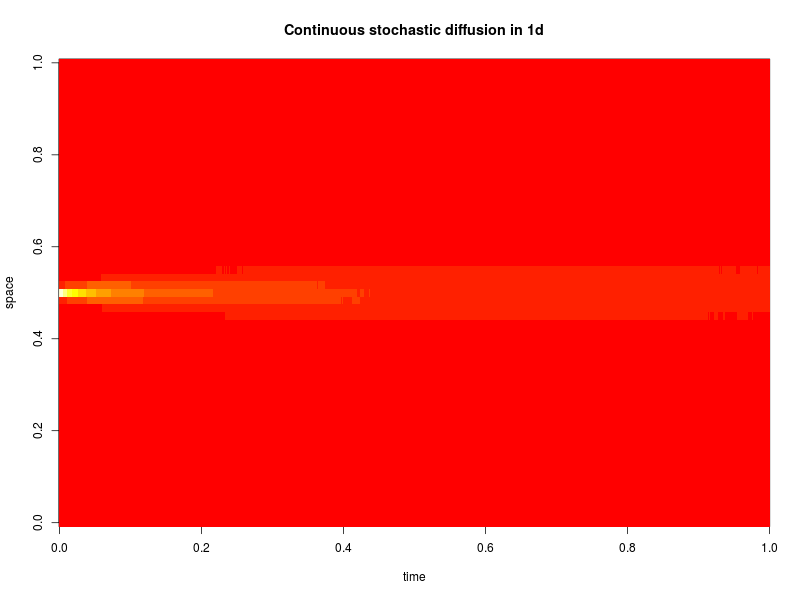
\includegraphics[height=0.8\textheight]{sgdiff1d}}
}

\frame{
\frametitle{Length scaling}
\begin{itemize}
\item The rate at which molecules move from one subvolume to the next must obviously depend on the size of the box
\item The smaller the box, the higher the rate at which molecules diffuse out of the box
\item Thinking about random walks and the expected distance from the origin, it is clear that the rate must be proportional to \emph{length}${}^{-2}$, so put
\[
D = D_c / l^2,
\]
where $D_c$ is the continuum rate of diffusion and $l$ is the (cubic) length of the volume
\end{itemize}
}

\frame{
\frametitle{Continuum limit}
\begin{itemize}
\item The noise becomes negligible in high concentration scenarios
\item Setting the noise terms to zero gives
\[
\frac{d x_{i}}{d t} = D\Delta x_{i},\quad i=1,2,\ldots,N
\]
which corresponds exactly to the \alert{method of lines} for the \alert{centred finite difference} approximation to the heat/diffusion equation
\[
\frac{\partial x}{\partial t} = D_c\Delta x
\]
\item \alert{With} the noise terms, it is a method of lines approach to solving the relevant diffusion \alert{SPDE}
\end{itemize}
}


\frame{
\frametitle{Multivariate SDE}
Put $X_t = \begin{pmatrix}X_{1,t}\\X_{2,t}\\\vdots\\X_{N,t}\end{pmatrix}$,
\(
B = \begin{pmatrix}0&0&0&\cdots&0&1\\1&0&0&\ddots&0&0\\0&1&0&\ddots&0&0\\\vdots&\ddots&\ddots&\ddots&\ddots&\vdots\\0&0&0&\cdots&1&0\end{pmatrix}
\),
$\nabla=I-B$, $\Delta=\nabla^2B^{-1}=\nabla^2B\trans$, so that
\[
\Delta = \begin{pmatrix}-2&1&0&0&\cdots&0&1\\1&-2&1&0&\ddots&0&0\\0&1&-2&1&\ddots&0&0\\\vdots&\ddots&\ddots&\ddots&\ddots&\ddots&\vdots\\0&0&0&0&\ddots&-2&1\\1&0&0&0&\cdots&1&-2\end{pmatrix}
\]
}

\frame{
\frametitle{Multivariate SDE}
\begin{itemize}
\item Clear we can write the drift as $D\Delta X_t$
\item Elementary manipulation gives the ``diffusion'' matrix as $\sqrt{D}\nabla\operatorname{diag}\{\sqrt{(I+B\trans)X_t}\}$
\item Then we can describe diffusion on the lattice with the multivariate SDE
\begin{block}{Lattice diffusion as a multivariate SDE}
\[
dX_t = D\Delta X_t\,dt +  \sqrt{D}\nabla\operatorname{diag}\left\{\sqrt{(I+B\trans)X_t}\right\}\,dW_t
\]
\end{block}
\item Clear to SPDE experts that this is a method of lines solution to a limiting SPDE
\end{itemize}
}

\subsection{Stochastic reaction diffusion on a 1D lattice}


\frame{
\frametitle{Reaction diffusion master equation (RDME)}
\begin{itemize}
\item Returning to the discrete stochastic case, let's now consider multiple species and additional reactions...
\item For the Lotka Volterra model, we just have separate species for the prey and predator in each subvolume
\begin{align*}
X_i &\longrightarrow 2X_i \tag{prey reproduction}\\
X_i+Y_i &\longrightarrow 2Y_i \tag{prey-predator interaction}\\
Y_i &\longrightarrow \emptyset \tag{predator death} \\
X_i &\longrightarrow X_{i+1} \tag{prey moves right} \\
X_i &\longrightarrow X_{i-1} \tag{prey moves left} \\
Y_i &\longrightarrow Y_{i+1} \tag{predator moves right} \\
Y_i &\longrightarrow Y_{i-1} \tag{predator moves left}
\end{align*}
\item So in this case we now have 2 species and 7 reactions per box
\end{itemize}
}

\frame{
\frametitle{Discrete stochastic Lotka Volterra on a 1d lattice}
Just simulate trajectories with the Gillespie algorithm:
\centerline{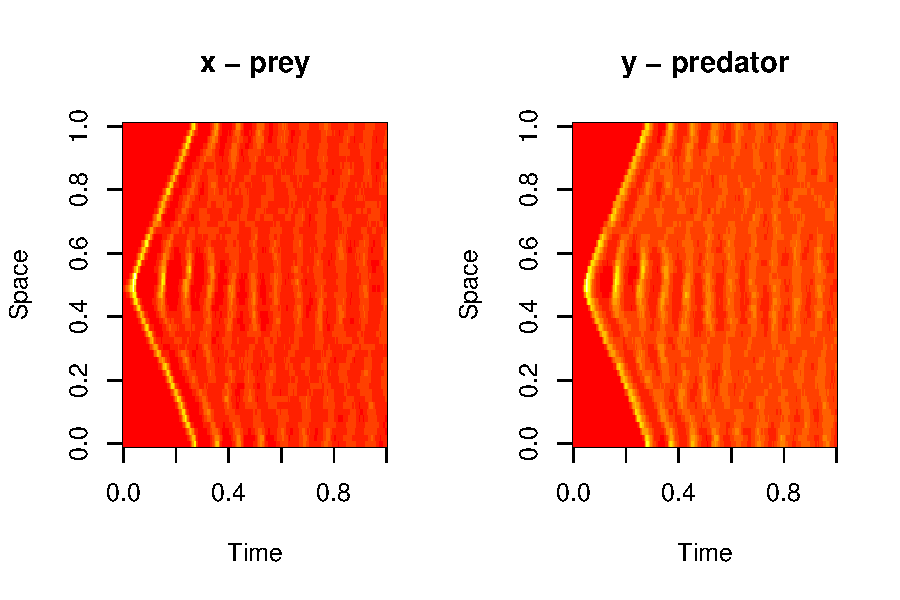
\includegraphics[height=0.8\textheight]{dsrd1d}}
}

\frame{
\frametitle{RDME}
\begin{itemize}
\item The chemical master equation (CME) in the well mixed case is
\[
\frac{d}{dt}p(x,t) = \sum_{j=1}^v \left[ h_j(x-S^{(j)})p(x-S^{(j)},t) - h_j(x)p(x,t) \right]
\]
\item If we now let $X$ be a $u\times N$ matrix of molecule counts, with elements $x_{ij}$, then the RDME can be written
\end{itemize}
\begin{multline*}
\frac{d}{dt}p(X,t) = \\ \sum_{n=1}^N \sum_{m\in\{n-1,n+1\}} \sum_{i=1}^u D_i\left[ (x_{im}+1)p(X+\delta_{im}-\delta_{in},t) - x_{im}p(X,t) \right] \\
+ \sum_{n=1}^N \sum_{j=1}^v \left[ h_j(X^{(n)}-S^{(j)})p(X-S^{(j)}e_n\trans,t) - h_j(X^{(n)})p(X,t) \right]
\end{multline*}
}

\frame{
\frametitle{Next subvolume method}
\begin{itemize}
\item The model ends up being a Markov jump process and so can be simulated with any exact discrete event simulation algorithm --- the previous example was simulated using a simple Gillespie algorithm
\item Due to the large number of species, reactions and reaction events, naive implementations of the Gillespie algorithm are inefficient
\item The \alert{next subvolume method} (Elf and Ehrenberg, '04) is a variant of the \alert{next reaction method} (Gibson and Bruck, '00) for RDME models
\item The algorithm keeps track of the time of the next event for each subvolume in a queue, and then selects the next subvolume to have an event executed from the top of the queue
\end{itemize}
}

\frame{
\frametitle{Lotka-Volterra with 1D diffusion}
ONE OR TWO EXAMPLE PLOTS
}

\frame{
\frametitle{The spatial chemical Langevin equation (CLE)}
\small
\begin{itemize}
\item Start by thinking separately about diffusion and reaction --- $X_{i,n,t}$ is amount of species $i$ in subvolume $n$ at time $t$
\item Diffusion: $dX_{i,n,t} = D_i\Delta X_{i,n,t} dt + \sqrt{D_i}\left(\sqrt{(1+B^{-1})X_{i,n,t}} - \sqrt{(1+B)X_{i,n,t}}B\right)dW_{i,n,t}$
\item Reaction: $dX_{i,n,t} = S_ih(X_{n,t})dt+S_i\operatorname{diag}\left\{\sqrt{h(X_{n,t})}\right\}dW^\star_{n,t}$
\item Combining these gives the spatial CLE:
\end{itemize}
\begin{multline*}
dX_{i,n,t} = [D_i\Delta X_{i,n,t}  +S_ih(X_{n,t})]dt+ \sqrt{D_i}\left(\sqrt{(1+B^{-1})X_{i,n,t}} \right. \\ \left. - \sqrt{(1+B)X_{i,n,t}}B\right)dW_{i,n,t}+S_i\operatorname{diag}\left\{\sqrt{h(X_{n,t})}\right\}dW^\star_{n,t}
\end{multline*}
\begin{itemize}
\item But in practice, just alternate between diffusion and reaction steps for every species in every subvolume
\end{itemize}
}

\frame{
\frametitle{Spatial CLE for Lotka-Volterra}
ONE OR TWO EXAMPLE PLOTS
}

\frame{
\frametitle{Volume scaling}
\begin{itemize}
\item We have seen how the diffusion constants scale with the \alert{length} of the associated subvolume
\item Reaction rates for the well mixed case typically scale according to the \alert{volume} of the container, with the scaling depending on the order of the reaction
 \begin{itemize}
 \item Zeroth order: Stochastic rate $c_j = k_j V$ for volume-independent rate $k_j$ (typically)
 \item First order: Rates are independent of volume, $c_j = k_j$
 \item Second order: Stochastic rate $c_j = k_j / V$ is inversely proportional to the container volume
 \end{itemize}
\item By scaling rates appropriately, we can simulate model on coarser and finer grids without changing qualitative behaviour (up to a point)
\end{itemize}
}

\frame{
\frametitle{Spatial CLE on a fine grid}
EXAMPLE PLOT
}

\section{Stochastic reaction diffusion in 2D}

\subsection{Diffusion in 2D}

\frame{
\frametitle{Discrete stochastic diffusion on a 2d lattice}
}

\frame{
\frametitle{Isotropy and lattice artifacts}
}

\frame{
\frametitle{SDE approximation}
}

\subsection{Reaction diffusion in 2D}

\frame{
\frametitle{Lotka Volterra in 2d}
\begin{itemize}
\item blah
\end{itemize}
}

\frame{
\frametitle{Discrete stochastic reaction diffusion on a 2D lattice}
\begin{center}
%\includemovie{.8\textheight}{.8\textheight}{dsrd2d.mp4}
\movie[externalviewer]{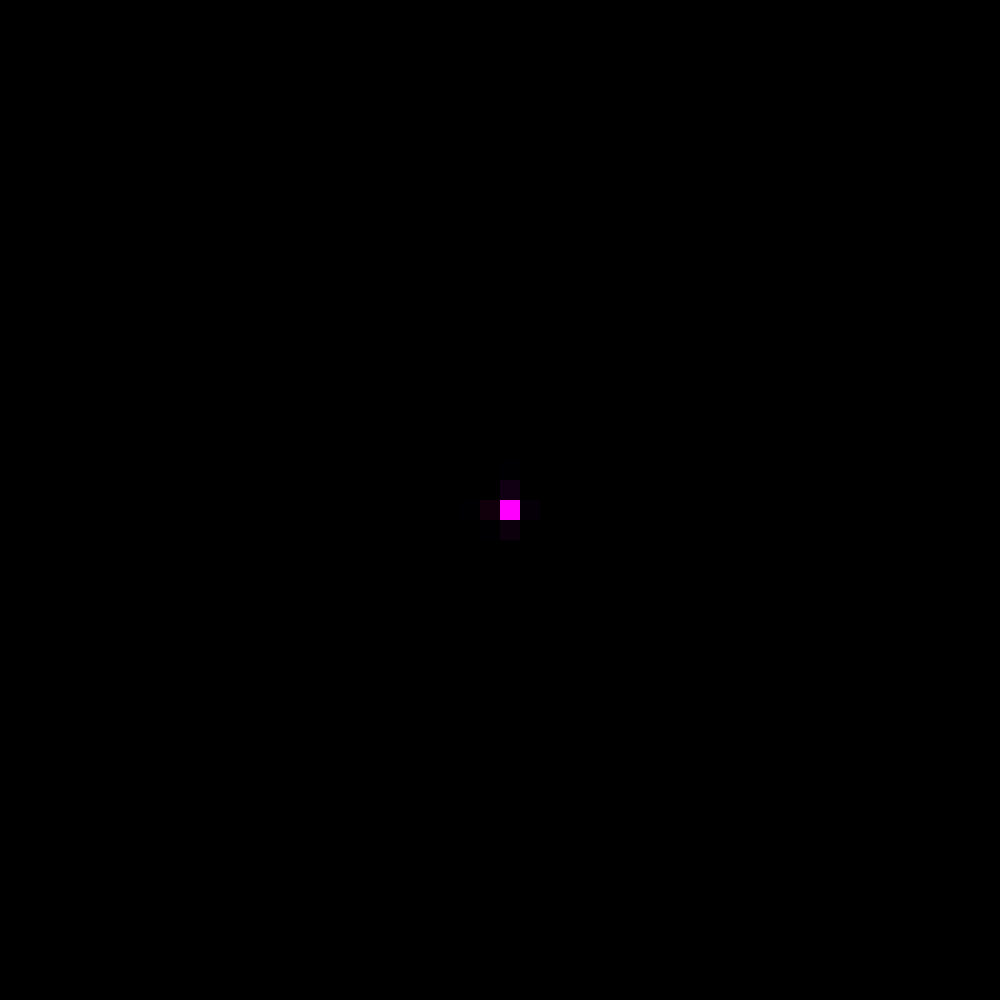
\includegraphics[height=0.8\textheight]{dsrd2d}}{dsrd2d.mp4}
\end{center}
}

\frame{
\frametitle{SDE approximaton}
}


\frame{
\frametitle{blah}
\begin{itemize}
\item blah
\end{itemize}
}


\frame{
\frametitle{blah}
\begin{itemize}
\item blah
\end{itemize}
}


\end{document}

